\documentclass[a4paper,16pt]{article}
\usepackage[utf8]{inputenc}
\usepackage{enumitem}
\usepackage{amsmath}
\usepackage{tikz}
\usepackage{tkz-tab}
\usepackage{caption}
\usepackage{latexsym}
\usepackage{amssymb}
\usepackage{amsmath}
\usepackage{subcaption} 
\usepackage{float}
\usetikzlibrary{positioning} 
\usepackage{graphicx, subfig}
\usepackage{algorithm}
\usepackage{algorithmic}
\usepackage{color}

\newcommand{\argmin}{\arg\!\min}
\newcommand{\argmax}{\arg\!\max}
\newcommand{\red}[1]{\textcolor{red} {#1}}

\newcommand{\todo}{\red{TODO }}

% Add 1cm of margin to left and rigth side
\addtolength{\textwidth}{3cm}
\addtolength{\hoffset}{-1.5cm}

\setlist{listparindent=\parindent}

\author{Eliel Hojman - elielhs - 332694868}
\title{Medical Image Processing, Exercise 2}


%\begin{figure}[H]
%	\centering
%	\begin{minipage}[b]{0.6\linewidth}
%        \includegraphics[width=\linewidth]{component_graph.jpg}
%	\end{minipage}
%	\caption{Number of components for each i\_min value}
%\end{figure}


\begin{document}
\maketitle

\section{Part 1 - Registration based on hand selected points of interest}

\begin{enumerate}
\item Below can be seen both images used for the registration as well as the 10 point of interest selected. 
\begin{figure}[H]
	\centering
	\begin{minipage}[b]{0.99\linewidth}
        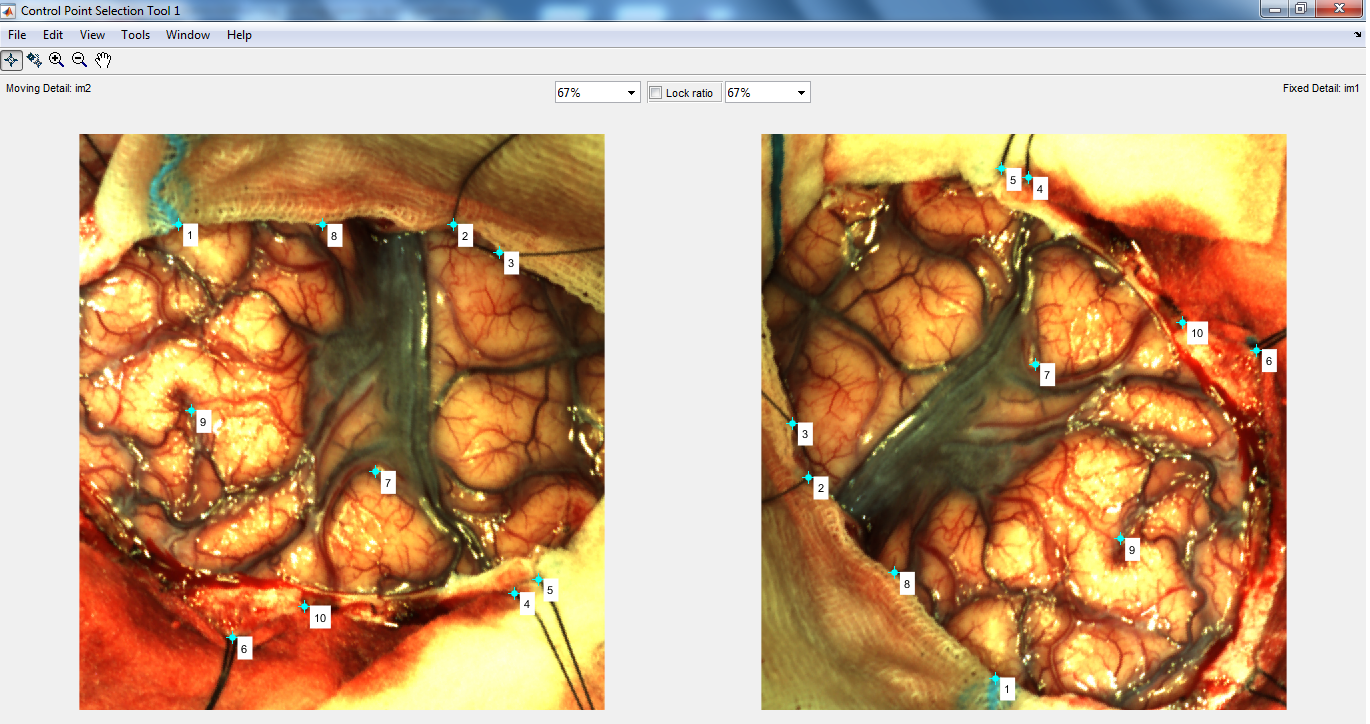
\includegraphics[width=\linewidth]{selectingPoints.png}
	\end{minipage}
	\caption{Hand selected points of interest}
\end{figure}

\stepcounter{enumi}

\item For the points selected in part 1 we obtained a RSME error of $1.66$ pixels. Below we can see the same image as above with the 10th point moved to calculate the error in case of one outline. For this case the RSME result was of $26.11$, an error 15 times bigger than the previous one. The calculations to find the rotation matrix and traslation take into account all of the points, so it is important there are not many outliers, specially when we are working with a small number of points such as 10, as we are doing here. 

\begin{figure}[H]
	\centering
	\begin{minipage}[b]{0.99\linewidth}
        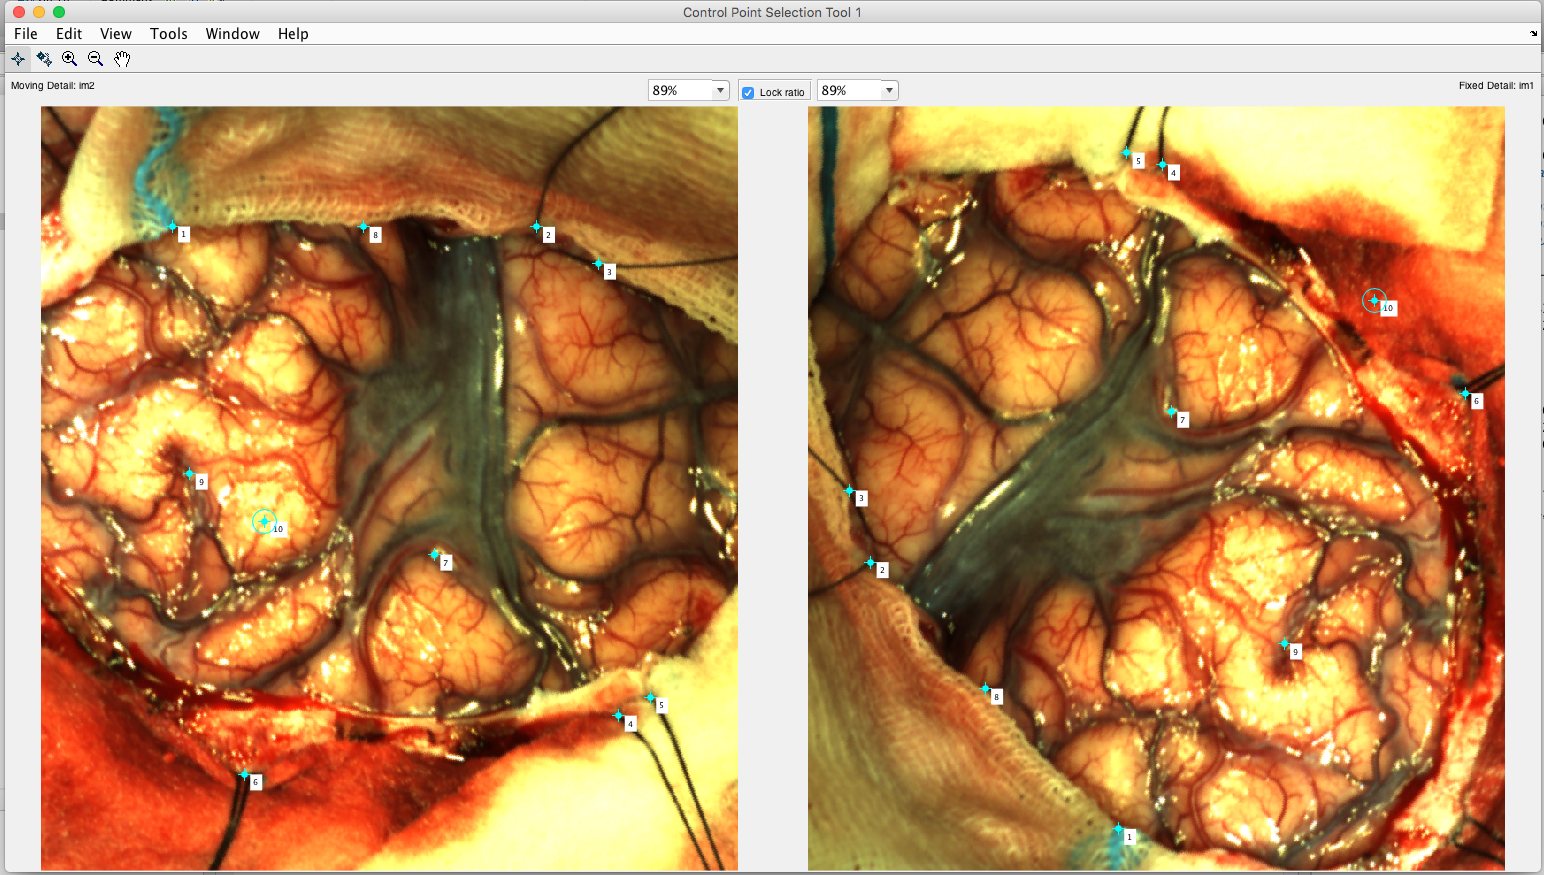
\includegraphics[width=\linewidth]{badPoints.png}
	\end{minipage}
	\caption{Hand selected points of interest}
\end{figure}

\item Below we can see the results of the registration. On the left image only the edges of one of the pictures is displayed. On the right both of the images are fully displayed. As it can clearly be seen we obtained very good results.

\begin{figure}[H]
	\centering
	\begin{minipage}[b]{0.45\linewidth}
        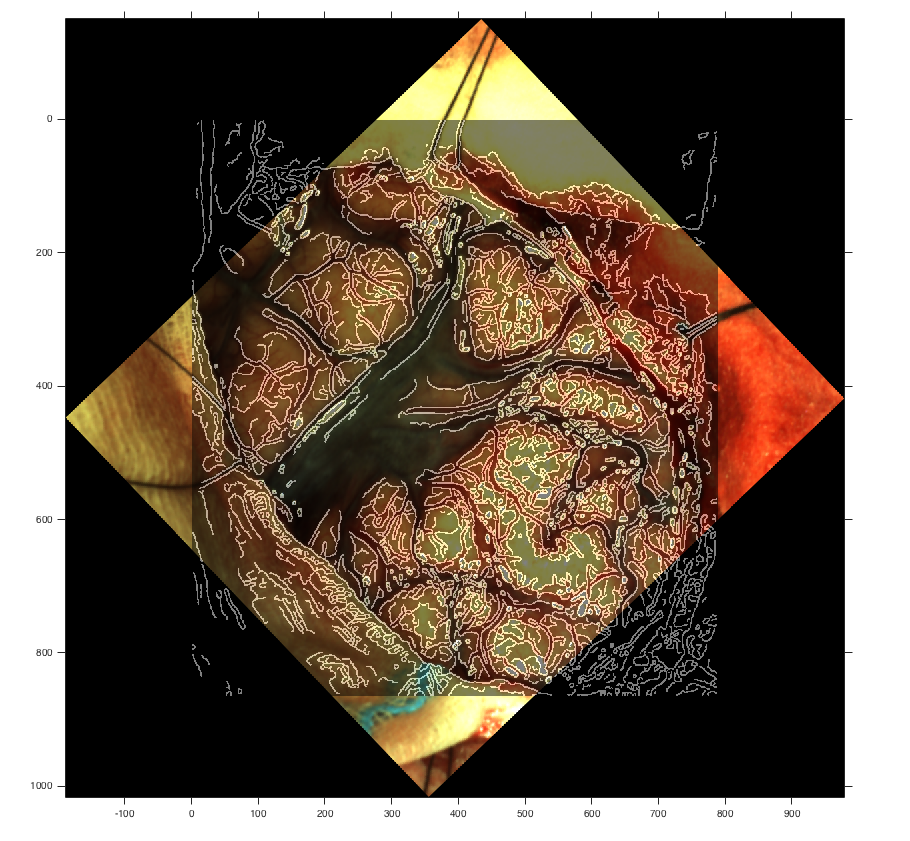
\includegraphics[width=\linewidth]{registrationEdges.png}
	\end{minipage}
	\begin{minipage}[b]{0.45\linewidth}
        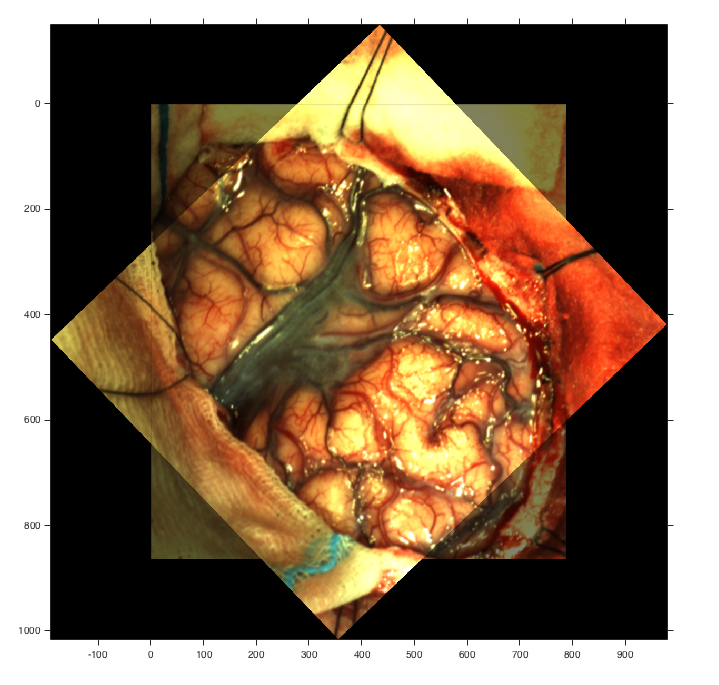
\includegraphics[width=\linewidth]{registrationImgs.png}
	\end{minipage}	
	\caption{Results of the registration}
\end{figure}

\end{enumerate}



\end{document}



